%%%%%%%%%%%%%%%%%%%%%%%%%%%%%%%%%%%%%%%%%%%%%%%%%%%%%%%%%%%%%%%%%%%%%%%%%%%%%%

\documentclass{l3deliverable}

%%%%%%%%%%%%%%%%%%%%%%%%%%%%%%%%%%%%%%%%%%%%%%%%%%%%%%%%%%%%%%%%%%%%%%%%%%%%%%

\usepackage{graphicx}%
%


\version{1.0}


\usepackage{tabularx}%
\usepackage{url}%
\usepackage{usecasedescription}%

%%%%%%%%%%%%%%%%%%%%%%%%%%%%%%%%%%%%%%%%%%%%%%%%%%%%%%%%%%%%%%%%%%%%%%%%%%%%%%
%% Check these macro values for appropriateness for your own document.

\title{Requirements Document}

\author{Michael Kilian\\
	Dan Tomosoiu\\
	Tony Lau\\
	Peeranat Fupongsiripan\\
	Hector Grebbel
}

\date{31 October 2012}

\deliverableID{D3}
\project{PSD3 Group Exercise 1}
\team{L}

%%%%%%%%%%%%%%%%%%%%%%%%%%%%%%%%%%%%%%%%%%%%%%%%%%%%%%%%%%%%%%%%%%%%%%%%%%%%%%

\begin{document}

%%%%%%%%%%%%%%%%%%%%%%%%%%%%%%%%%%%%%%%%%%%%%%%%%%%%%%%%%%%%%%%%%%%%%%%%%%%%%%

\maketitle

\tableofcontents

\newpage

%%%%%%%%%%%%%%%%%%%%%%%%%%%%%%%%%%%%%%%%%%%%%%%%%%%%%%%%%%%%%%%%%%%%%%%%%%%%%%
%% Standard section for all documents

\section{Introduction}
Software Engineering (SE) and Electronic and Software Engineering (ESE) students in the School
of Computing Science are required to complete an internship as part of their course, in the summer
between level 3 and level 4. An internship is a short period of time that a student spends working
within in a company in order to gain experience (from as little as a month up to a year). Internships
in the software industry are normally paid, although the rate offered can vary from company to
company. The School imposes requirements on these internships to ensure that the student receives
an appropriate experience for their degree programme. More details of these restrictions can be found
on the Software Engineering Summer Placement (SESP) moodle page.\\
\\
Currently, available internships are advertised to students on an ad-hoc basis through the SESP
moodle page. An organisation wishing to recruit an intern submits an advertisement to the course
coordinator, who publishes it on the course mailing list. The format and content of the advert can
vary widely, including information about the nature of the internship (what the successful applicant
will do), duration, expected start date, compensation, person requirements and so on. The course
coordinator checks each advert and comments on whether it is suitable for SE/ESE students, as students 
who are not enrolled on the SE/ESE scheme may also view the advertisements posted on
the SESP moodle page in order to obtain information about possible internships.\\
\\
Sometimes internships applications are managed through the Careers Service's Club21 website;
sometimes through the e-Placements scheme; and sometimes the company has its own system of
collecting applications. In addition, some advertisements are posted by academics in the school for
students to work with them during the summer vacation.\\
\\
The allocation of SE/ESE students to internships is tracked by the course coordinator separately,
using a Microsoft Access Database. Students are required to inform the coordinator when they have
secured a placement, which may or may not have been advertised on the SESP page. The coordinator
must then approve the internship if it is suitable for the student's course.\\
\\
The SESP course coordinator has decided that a unified system is necessary for collecting and
publishing internship advertisements, and for tracking which SE/ESE students have been successful
in securing them. An initial requirements analysis has found that the following features must be
supported by the system:
\begin{itemize}
\item{Submission of internship advertisements}
\item{Review, comment and publication of internship advertisements by the course coordinator}
\item{Review of advertisements by students}
\item{Notification of successful selection for an internship by an SE/ESE student}
\end{itemize}
\subsection{Identification}

\subsection{Related Documentation}
\begin{itemize}
\item{Client interview questions}
\item{Raw requirements list}
\end{itemize}

\subsection{Purpose and Description of Document}
This document displays the use cases we have identified for the system. The long term aim of the document is to add to it as new requirements are identified and to use it
as a basis for system design. 
\subsection{Document Status and Schedule}
This document should be revised weekly at the very least and ideally should be updated whenever a new use case is identified or is deemed important enough to implement.

%%%%%%%%%%%%%%%%%%%%%%%%%%%%%%%%%%%%%%%%%%%%%%%%%%%%%%%%%%%%%%%%%%%%%%%%%%%%%%
\newpage
\section{Extended Problem Defintion}

\newpage
\section{System Scope}
As specified in the initial business case, the system is only to be used within the department of computing science. The only outside interaction comes from companies who
submit advertisements to the system. \\
The process of a student applying for a placement is the most complex with regards to scope. In many cases larger companies will have their own websites or online application
processes which they will wish the student to take part in. In this case the student does not apply through the system and will aplly by using the details found in the corresponding
advert for the placement. However smaller, independant companies may not have their own process. For such companies the system will handle direct applications by the student to 
the company.Finally the student may also find placements entirely on their own. When this occurs the student should submit information about the placement through the system, but
the application to the placement is outside the system scope.
\\

%%%%%%%%%%%%%%%%%%%%%%%%%%%%%%%%%%%%%%%%%%%%%%%%%%%%%%%%%%%%%%%%%%%%%%%%%%%%%%

\subsection{System Actors}
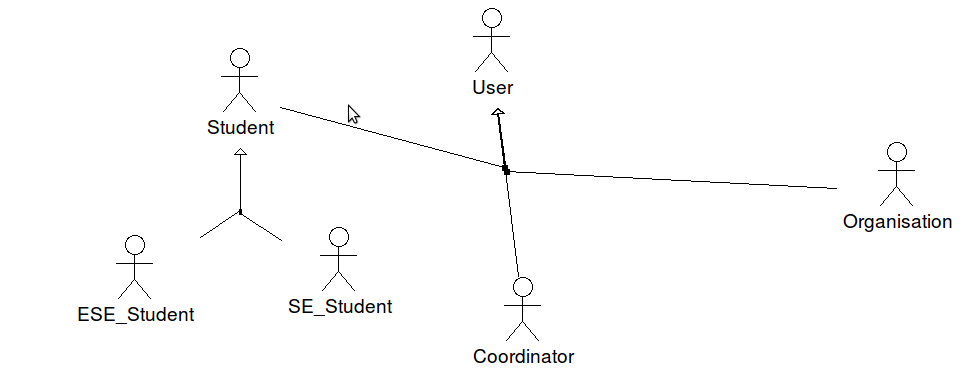
\includegraphics[scale = 0.5]{Actors.png}

The above diagram shows the actor roles present in the system:
\begin{itemize}
\item{\textbf{Student:}\ all students enrolled in the system who can apply for placements. This can be further broken down into SE and ESE students, who will have
different rules on what constitues a suitable placment.}
\item{\textbf{Coordinator: }\ the course coordinator will have privileges to approve and reject files, view student progress, etc.}
\item{\textbf{Organisation: }\ any group who advertises placements to the system. This may include external companies, intership schemes and university groups.}
\end{itemize}
%%%%%%%%%%%%%%%%%%%%%%%%%%%%%%%%%%%%%%%%%%%%%%%%%%%%%%%%%%%%%%%%%%%%%%%%%%%%%%

\subsection{Domain Model}
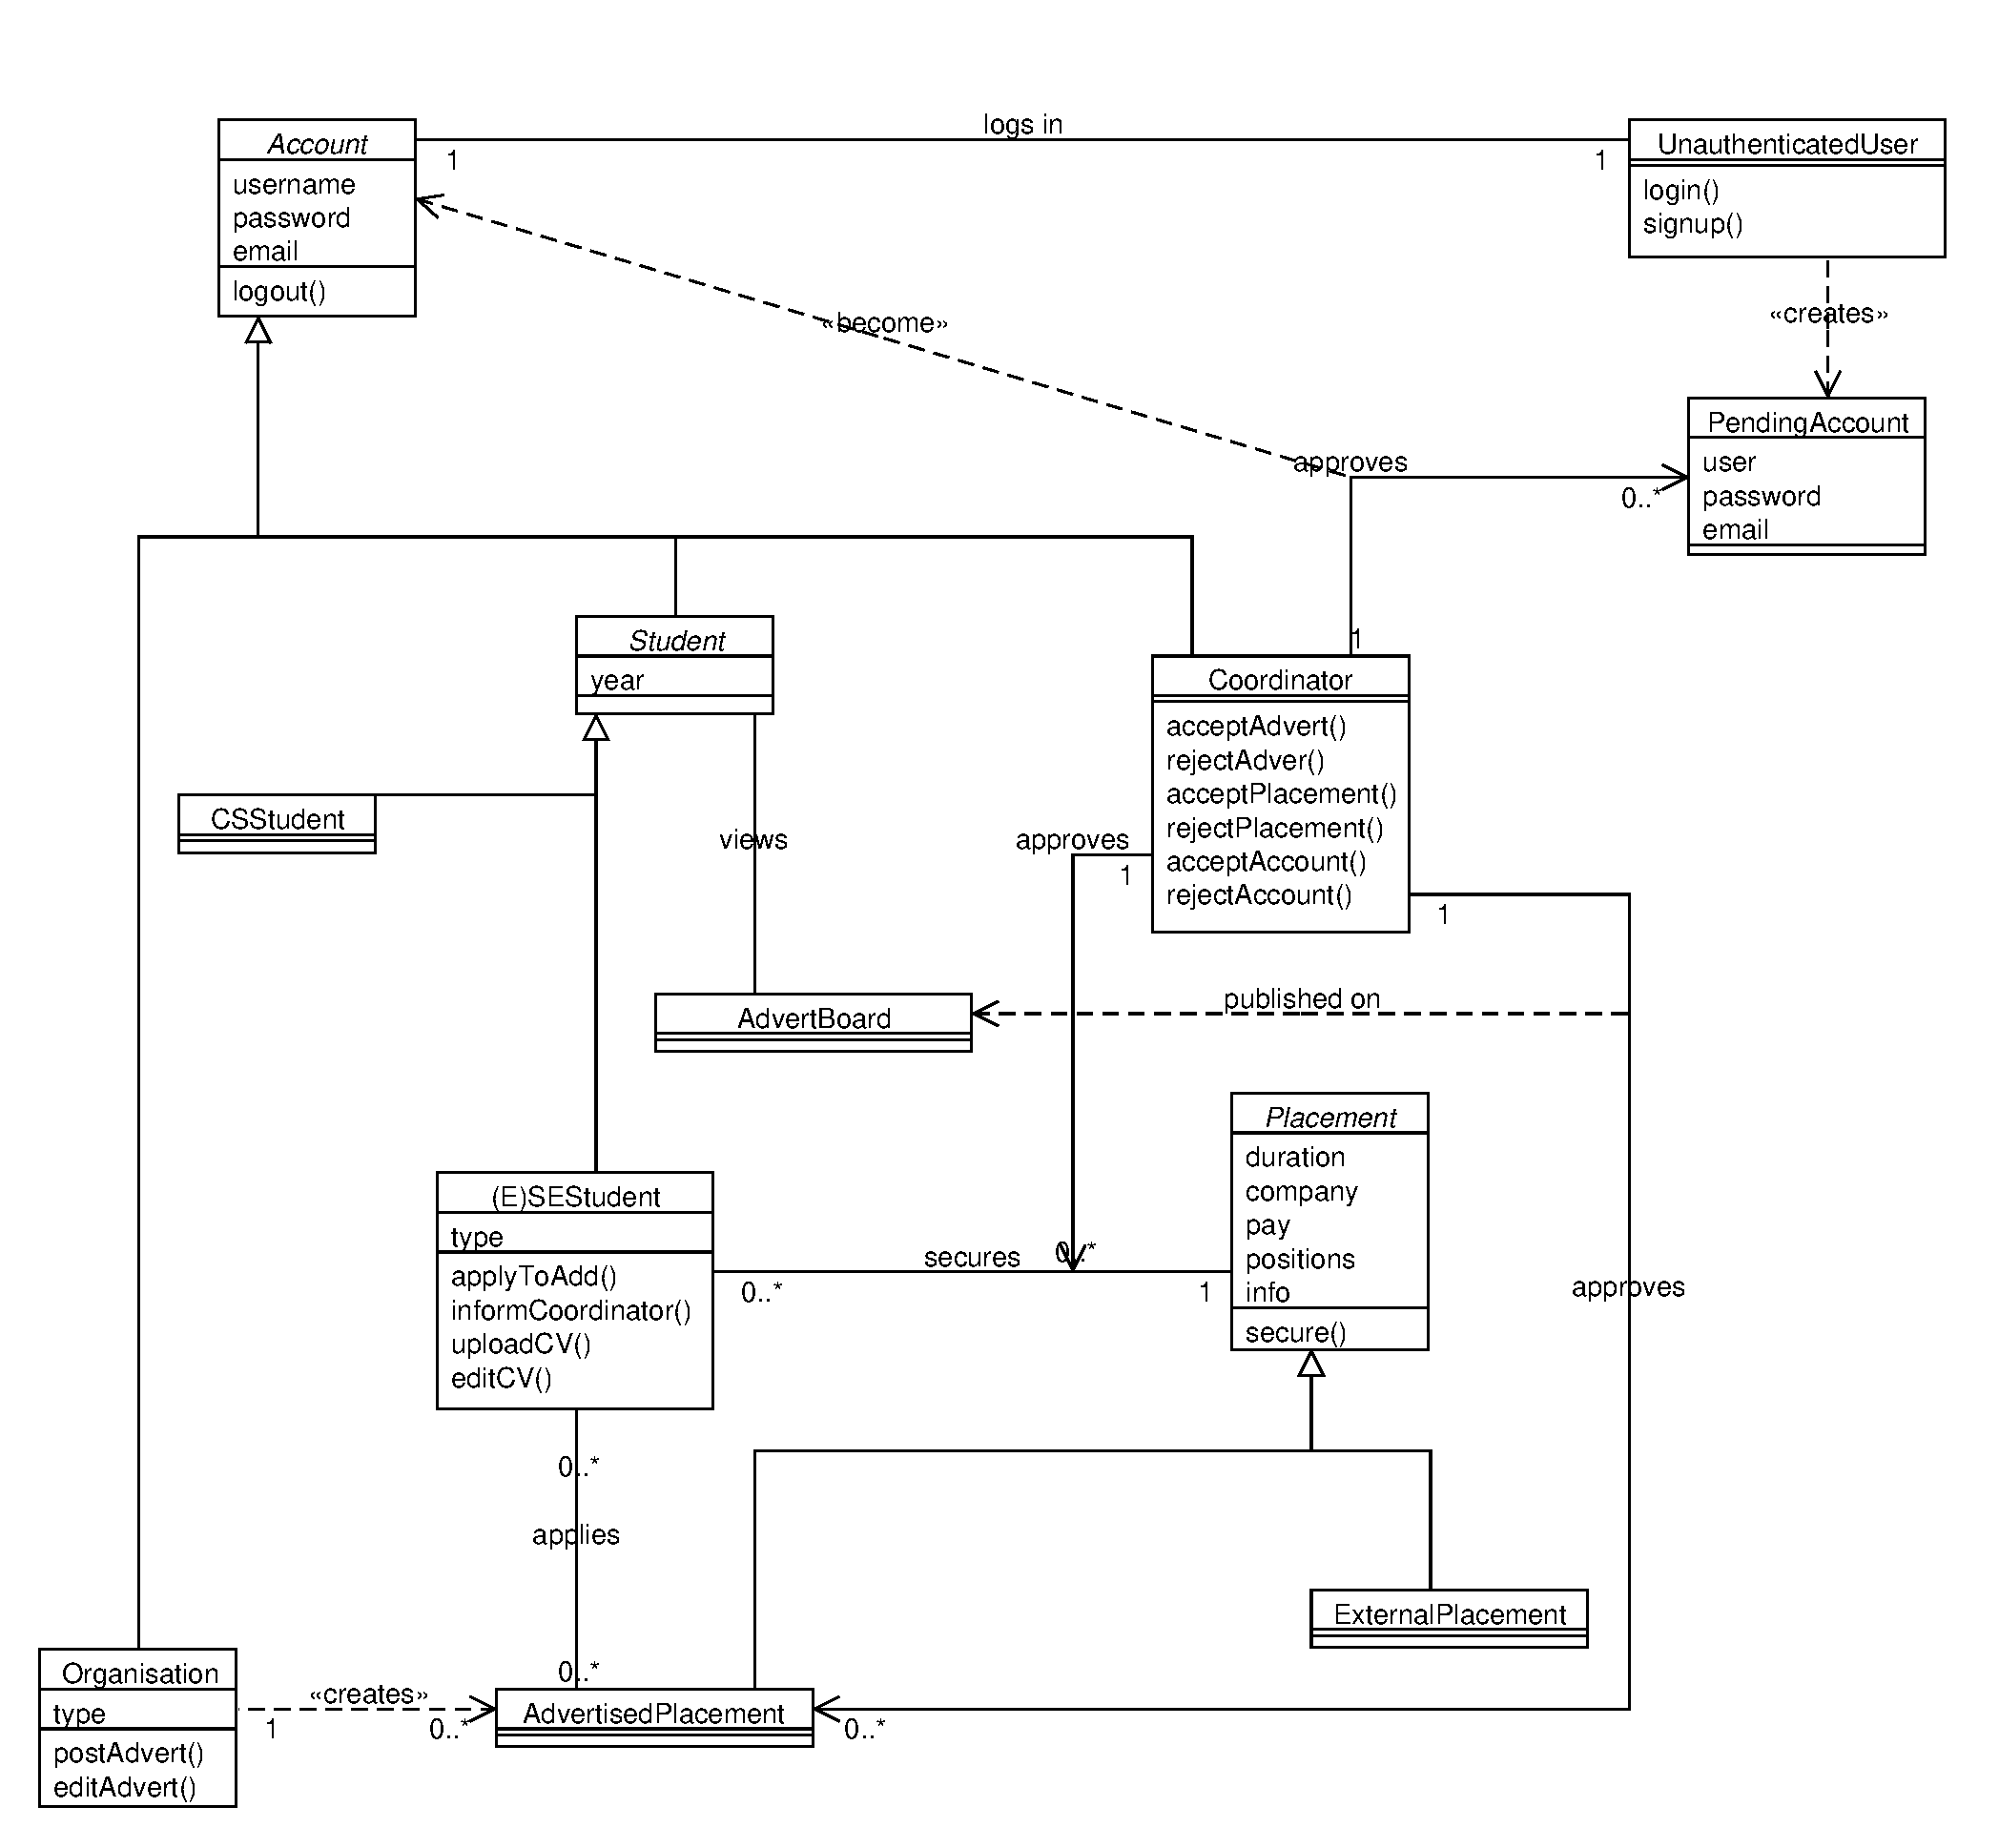
\includegraphics[scale=0.45]{domain_model_v2.pdf}\\
Unauthenticated users represents the guests that visit the system, prior to logging in.\\\
Unauthenticated users can opt to sign up, which creates a PendingAccount instance, that needs to be approved by a Coordinator. Once the Coordinator approves it, the PendingAccount becomes one of the three types of Account, and can then be used for logging in.\\

Account is a generalisation representing user accounts. This branches off to three types of account - Organisation, Coordinator and Student.\\

Organisations represent either Companies or Academics (distinguished by type). They create AdvertisedPlacements that, once approved by a Coordinator, become visible on the AdvertBoard.\\

Students are either ordinary Computing Science students, in which case they can only view adverts, or (Electronic) Software Engineering students, which can also apply to the placements that are visible on the Advert Board.\\

Students can secure placements, either from the ones visible on the AdvertBoard, or from external sources. Coordinators need to approve the securing of placements.


%%%%%%%%%%%%%%%%%%%%%%%%%%%%%%%%%%%%%%%%%%%%%%%%%%%%%%%%%%%%%%%%%%%%%%%%%%%%%%
\newpage
\section{Use Case Descriptions}
This section describes the key features which are required for the system. These can be broken into four categories as follows:\
\begin{itemize}
\item{\textbf{Utilities / Account Management}
	\begin{itemize}
		\item{Login}
		\item{Account Creation}
		\item{Company Account Creation}
	\end{itemize}
	\textbf{Coordinator Administration}
	\begin{itemize}
		\item{Advert Approval}
		\item{Mark placements as filled}
	\end{itemize}
	\textbf{Advert Submission}
	\begin{itemize}
		\item{Submission of adverts by organisations}
		\item{Submission of external placements by students}
	\end{itemize}
	\textbf{Advert viewing and applications}
	\begin{itemize}
		\item{Viewing of adverts}
		\item{Application for placement through system}
		\item{Notification of successfully securing a placement}
	\end{itemize}
\end{itemize}
\newpage
\subsection{Utilities / Account Management}
\begin{UseCaseTemplate}
\UseCaseLabel{Login}
\UseCaseDescription{User logs in to system to be recognised and allow them to perform role specific actions}
\UseCaseRationale{Identified a need for different classes of user to have a different range of functionality presented. For example only the coordinator should be able to approve adverts.}
\UseCasePriority{Must Have}
\UseCaseActors{All}
\UseCaseExtensions{}
\UseCaseIncludes{}
\UseCaseConditions{\textbf{pre}\ user must have an account created in the system}
\UseCaseNonFunctionalRequirements{Email details when details are lost.}
\UseCaseScenarios{\begin{itemize}
\item{\textbf{Primary:}\ Mark enters his username and password into the corresponding fields and selects login. He is logged into the system successfully.}
\item{\textbf{Alternate 1:}\ Ross makes a typing mistake whilst entering his password and attempts to login. The system reports this error and prompts him to reenter his password.}
\item{\textbf{Alternate 2:}\ Craig wishes to login to the system but has forgotten his details. He chooses to have his password sent to him. He enters his email to which the account is registered and selects send. Using
the details emailed to him he successfully logs in.}
\end{itemize}}
\UseCaseRisks{}
\UseCaseUserInterface{Username/Password input fields}
\end{UseCaseTemplate}

\begin{UseCaseTemplate}
\UseCaseLabel{Account Creation}
\UseCaseDescription{It must be possibe to create accounts on the system for all users. SE/ESE students have accounts created automatically.}
\UseCaseRationale{To interact on an individual basis with the system, it must have some way of telling who is using it}
\UseCasePriority{Must Have}
\UseCaseStatus{Not Implemented}
\UseCaseActors{Course Co-ordinator}
\UseCaseExtensions{Company Account Creation}
\UseCaseIncludes{}
\UseCaseConditions{\textbf{pre}\ Account ID does not already exist
\textbf{post}\ Account now present on system}
\UseCaseNonFunctionalRequirements{\begin{itemize}
\item{Security}
\item{Graphical User Interface}
\item{Account details are editable}
\end{itemize}
}
\UseCaseScenarios{
\begin{itemize}
\item{\textbf{Primary:}\ Course Co-Ordinator creates an account for a student}
\item{\textbf{Alternative 1:}\ Automatic Enrollment for SE/ESE Students}
\item{\textbf{Alternative 2:}\ Course Co-Ordinator creates an account for a company}
\end{itemize}
}
\UseCaseRisks{Account created with incorrect details}
\UseCaseUserInterface{A field based input for each value required}
\end{UseCaseTemplate}

\begin{UseCaseTemplate}
\UseCaseLabel{Company Account Creation}
\UseCaseDescription{A Company has an account, which allows them to submit adverts directly to the system for approval. It also allows students applications
to be forwarded directly.}
\UseCaseRationale{This saves the course co-ordinator time, since he does not have to manually enter each advert. It also means applications reach the companies more quickly.}
\UseCasePriority{Should Have}
\UseCaseActors{Coordinator\\
Organisation}
\UseCaseExtensions{}
\UseCaseIncludes{}
\UseCaseConditions{}
\UseCaseNonFunctionalRequirements{}
\UseCaseScenarios{
\begin{itemize}
\item{\textbf{Primary:}\ A Company Submits an advert to the system}
\item{\textbf{Alternate 1:}\ A Student submits an application to an advert. This is then sent to the company who placed it directly.}
\end{itemize}
}
\UseCaseRisks{This removes the ability for the couse co-ordinator to moderate students applications}
\UseCaseUserInterface{}
\end{UseCaseTemplate}
\newpage
\subsection{Coordinator Administration}
\begin{UseCaseTemplate}
\UseCaseLabel{Advert Approval}
\UseCaseDescription{The advert approval use case changes the status of an advert to approved ready to inform course students}
\UseCaseRationale{Course coordinator needs to be able to assess advert to be visible for course coordinator}
\UseCasePriority{Must Have}
\UseCaseStatus{Not Implemented}
\UseCaseActors{Coordinator}
\UseCaseExtensions{Email approved adverts to students}
\UseCaseIncludes{
\begin{itemize}
\item{Login}
\item{Viewing of adverts}
\end{itemize}
}
\UseCaseConditions{\textbf{pre} Advert must exist
\textbf{post} Advert is marked as approved and becomes viewable to students.}
\UseCaseNonFunctionalRequirements{Prompt for confirm before approving advert}
\UseCaseScenarios{\textbf{Primary:}\ John logs in and search for unapproved adverts on the advert board. He determines whether the advert is suitable for the course. Then, he marks the advert as approved. \textbf{Alternate 1:}\ Kate logs in and search for unapproved adverts. Then she accidentally click approve advert without determining the purpose of the course carefully.}
\UseCaseRisks{Advert may be accidentally approved before editing is complete or when advert is unsuitable.}
\UseCaseUserInterface{}
\end{UseCaseTemplate}

\begin{UseCaseTemplate}
\UseCaseLabel{Mark placements as filled}
\UseCaseDescription{User logs in to system and moves to view the advert board. They select their target application and mark it as taken by a student.}
\UseCaseRationale{There is obviously a need to communicate that a placement has been successfully filled so that other students dont waste their time making applications 
to it. However the client requested that in this situation the advert should not be removed, in case the placement becomes available again.}
\UseCasePriority{Should Have}
\UseCaseActors{Coordinator}
\UseCaseExtensions{}
\UseCaseIncludes{Viewing of Adverts}
\UseCaseConditions{
\textbf{pre}\ an advert exists for a placement which a student has filled 
\textbf{post}\ this advert is marked as taken
}
\UseCaseNonFunctionalRequirements{Persistence of advert after marking it as filled}
\UseCaseScenarios{
\begin{itemize}
\item{\textbf{Primary:}\ Valerie logs in and has a placement she wishes to mark as fulfilled by a student. She scrolls through the advert board until she finds
the advert, selects in and chooses an option to mark it as taken.}
\item{\textbf{Alternate 1:}\ Margaret logs in and searches the advert board for a placement she wishes to mark as taken. She mistakenly selects the wrong placement and proceed to mark it as taken.
Upon realising her mistake, she reselects the advert and chooses to reopen the advert for submissions.}
\end{itemize}
}
\UseCaseRisks{User could mistakenly mark an advert as taken and leave the system, making the advert appear closed to students ( and therfore most likely leave a taken advert
marked as unfulfilled), failing to notice their mistake.}
\UseCaseUserInterface{}
\end{UseCaseTemplate}


\newpage
\subsection{Advert Submission}
\begin{UseCaseTemplate}
\UseCaseLabel{Submission of adverts by organisation}
\UseCaseDescription{Companies, and academics in the university need to be able to submit advertisments for internships. This allows an organisation to submit an advertisement for an internship without emailing the course coordinator directly.}
\UseCaseRationale{This is a core feature of the system. It was originally specified in the business case}
\UseCasePriority{Must Have}
\UseCaseStatus{Not Implemented}
\UseCaseActors{Organisation}
\UseCaseExtensions{}
\UseCaseIncludes{Login}
\UseCaseConditions{
\textbf{pre}\ The organisation must have already obtained a login for the system. The organisation must be logged in.
\textbf{post}\ The advert is queued to be reviewed by the course coordinator before being visible to the users of the system
}
\UseCaseNonFunctionalRequirements{Structured input form}
\UseCaseScenarios{
\textbf{Primary:}\ Apple Inc. logs in successfully. They select the ‘Submit Advertisement’ menu item and are taken to the correct page. They fill in all fields and click the ‘Confirm’ button at the bottom of the page. A confirmation is displayed saying that the advert submission was successful.
\
\textbf{Alternate 1:} Dr. Jones logs in successfully. He selects the ‘Submit Advertisement’ menu item and is taken to the correct page. He enters details in the fields and clicks ‘Confirm’. An error message is displayed saying that not all fields have been filled out. Dr. Jones fill in the missing fields and clicks ‘Confirm’ again. A confirmation is displayed saying the advert submission was successful.\\
}
\UseCaseRisks{}
\UseCaseUserInterface{}
\end{UseCaseTemplate}


\begin{UseCaseTemplate}
\UseCaseLabel{Submission of external placement by SE/ESE student}
\UseCaseDescription{An SE/ESE student submits an advertisement for an internship not already advertised on system}
\UseCaseRationale{An SE/ESE student must get an internship approved by submitting the internship details}
\UseCasePriority{Should Have}
\UseCaseActors{Student}
\UseCaseExtensions{}
\UseCaseIncludes{Login}
\UseCaseConditions{
\textbf{pre}\ The student must have already obtained a login for the system (by automatic assignment or from the course coordinator). The student must be logged in.
\textbf{post}\ The advert is queued to be reviewed by the course coordinator
}
\UseCaseNonFunctionalRequirements{Structured input form}
\UseCaseScenarios{
\textbf{Primary:}\ Barry wants to submit an advert to be reviewed. He logs in to the system, clicks the submit advert button under the review section and fills in the details. It gives him a message confirming of success.\
}
\UseCaseRisks{}
\UseCaseUserInterface{}
\end{UseCaseTemplate}


\newpage
\subsection{Advert viewing and applications}


\begin{UseCaseTemplate}
\UseCaseLabel{Viewing of Adverts}
\UseCaseDescription{All users of the system must be able to view the advert board to review
adverts. This may only show a subset of the all adverts depending on the users status}
\UseCaseRationale{Fundamental to system description. Initial need specified in business case and exact method for viewing adverts elaborated in client interviews}
\UseCasePriority{Must Have}
\UseCaseStatus{Not Implemented}
\UseCaseActors{\begin{itemize}
\item{Organisation}
\item{Student}
\item{Coordinator}}
\UseCaseExtensions{}
\UseCaseIncludes{Login}
\UseCaseConditions{None}
\UseCaseNonFunctionalRequirements{}
\UseCaseScenarios{\textbf{Primary:}\ John logs in and attempts to find a suitable placement on the advert board. He scrolls down through the advert board until he finds a 
suitable placement, or there are no adverts left to view. He closes the interface.}
\UseCaseRisks{}
\UseCaseUserInterface{}
\end{UseCaseTemplate}

\begin{UseCaseTemplate}
\UseCaseLabel{Application for placement through system}
\UseCaseDescription{User logs in and finds the advert they wish to apply for. They click onto the advert and select the option to apply through the system. They are presented
with an interface through which they make their submission using their details and being allowed to attach any additional information. They then submit the application}
\UseCaseRationale{Some smaller companies may not have their own application process so in this scenario, the client has expressed a preference for applications to be handled
through the system.}
\UseCasePriority{Should Have}
\UseCaseStatus{Not Implemented}
\UseCaseActors{Student}
\UseCaseExtensions{}
\UseCaseIncludes{Viewing of Adverts}
\UseCaseConditions{\textbf{post}\ application has been submitted and made visible to company}
\UseCaseNonFunctionalRequirements{Structured input form}
\UseCaseScenarios{
\begin{itemize}
\item{\textbf{Primary:}\ Karl wishes to submit an application for an advert a friend told him about. He finds the advert on the board and chooses to submit
an application. He enters all relevant extra data and sends off the application. He exits the system.}
\item{\textbf{Alternate 1:} Ian selects an advert and chooses to submit an application. When prompted to enter any extra details he accidentally clicks send. He is prompted to 
confirm he wishes to submit the application. Thanks to this warning he recovers the error and enters data. He submits the application
}
\end{itemize}
}
\UseCaseRisks{Student could send away incomplete or erroneous applications accidentally. No method exists to retrieve/edit such an application}
\UseCaseUserInterface{}
\end{UseCaseTemplate}

\begin{UseCaseTemplate}
\UseCaseLabel{Notification of successfully securing a placement}
\UseCaseDescription{User logs in and chooses the relevant placement. He chooses to submit a message that he has been accepted for the placement. He includes any relevant info and sends the message.}
\UseCaseRationale{Course coordinator must ensure that every course student has their work placement.}
\UseCasePriority{Should Have}
\UseCaseActors{Student}
\UseCaseExtensions{}
\UseCaseIncludes{Login}
\UseCaseConditions{
\textbf{pre} - Advert must exist 
\textbf{pre} - Advert must be approved by course coordinator \textbf{pre} - Organisation has to secure the placement position for student 
\textbf{post} - course student's status is marked as secure}
\UseCaseNonFunctionalRequirements{}
\UseCaseScenarios{\textbf{Primary:}\ Andrew logs in and look for desirable and approved advert. He clicks on secure the placement button and sends an email about the selected placement to course coordinator.\textbf{Alternate 1:}\ Margaret logs in and select desirable advert but she cannot click on secure the placement button because the organisation she applies for has not accepted her position.}
\UseCaseRisks{It may take time for the organisation to secure student's position.}
\UseCaseUserInterface{}
\end{UseCaseTemplate}


%%%%%%%%%%%%%%%%%%%%%%%%%%%%%%%%%%%%%%%%%%%%%%%%%%%%%%%%%%%%%%%%%%%%%%%%%%%%%%
\newpage
\section{Non Functional Requirements}
No non functional requirements for the system as a whole have been identified to date. This should be a priority in the next requirements gathering phase.


%%%%%%%%%%%%%%%%%%%%%%%%%%%%%%%%%%%%%%%%%%%%%%%%%%%%%%%%%%%%%%%%%%%%%%%%%%%%%%

\section{Summary}

%%%%%%%%%%%%%%%%%%%%%%%%%%%%%%%%%%%%%%%%%%%%%%%%%%%%%%%%%%%%%%%%%%%%%%%%%%%%%%

\appendix


\section{Glossary}


\section{Scenarios}


\section{Stakeholder Interview Documentation}
These documents are available in our team repository:
\begin{itemize}
	\item{Client interview questions}
	\item{Interview audio recording}
	\item{Client consent form}
\end{itemize}




%%%%%%%%%%%%%%%%%%%%%%%%%%%%%%%%%%%%%%%%%%%%%%%%%%%%%%%%%%%%%%%%%%%%%%%%%%%%%%

\end{document}

%%%%%%%%%%%%%%%%%%%%%%%%%%%%%%%%%%%%%%%%%%%%%%%%%%%%%%%%%%%%%%%%%%%%%%%%%%%%%%
